\begin{table}[t]
\centering\small
\caption{Ablations of WHY (paired differences from the full method, 20 seeds, mean $\pm$ 95\% CI). Negative values mean the component helps. Poison share: percentage points of durable memory at night 34.}
\label{tab:ablation}
\begin{tabular}{@{}lcccc@{}}
\toprule
& Realistic & \multicolumn{3}{c}{Poisoning} \\
\cmidrule(lr){2-2}\cmidrule(lr){3-5}
Variant & $\Delta$ decision quality & $\Delta$ quality, nights 25--44 & $\Delta$ poison share & $\Delta$ ECE$^\ast$\\
\midrule
without Surprise $S$ & +0.004{\scriptsize$\,\pm$0.004} & +0.015{\scriptsize$\,\pm$0.006} & $-$1.9{\scriptsize$\,\pm$0.5} & $-$0.091{\scriptsize$\,\pm$0.007}\\
without Consequence $C$ & 0.000{\scriptsize$\,\pm$0.003} & +0.008{\scriptsize$\,\pm$0.005} & $-$3.5{\scriptsize$\,\pm$0.6} & +0.033{\scriptsize$\,\pm$0.009}\\
without Causal confidence $K$ & $-$0.015{\scriptsize$\,\pm$0.006} & $-$0.008{\scriptsize$\,\pm$0.007} & $-$0.7{\scriptsize$\,\pm$0.5} & +0.027{\scriptsize$\,\pm$0.008}\\
without Transferability $T$ & 0.000{\scriptsize$\,\pm$0.003} & +0.004{\scriptsize$\,\pm$0.004} & +0.6{\scriptsize$\,\pm$0.3} & +0.002{\scriptsize$\,\pm$0.003}\\
without Uncertainty reduction $U$ & $-$0.007{\scriptsize$\,\pm$0.004} & $-$0.009{\scriptsize$\,\pm$0.003} & $-$0.7{\scriptsize$\,\pm$0.4} & 0.000{\scriptsize$\,\pm$0.004}\\
without Manipulability discount & $-$0.021{\scriptsize$\,\pm$0.007} & $-$0.065{\scriptsize$\,\pm$0.012} & +12.4{\scriptsize$\,\pm$0.7} & +0.054{\scriptsize$\,\pm$0.007}\\
without retroactive tagging & $-$0.029{\scriptsize$\,\pm$0.008} & $-$0.029{\scriptsize$\,\pm$0.009} & $-$0.6{\scriptsize$\,\pm$0.4} & $-$0.017{\scriptsize$\,\pm$0.005}\\
without redundancy control & $-$0.004{\scriptsize$\,\pm$0.002} & +0.001{\scriptsize$\,\pm$0.004} & $-$0.3{\scriptsize$\,\pm$0.2} & $-$0.002{\scriptsize$\,\pm$0.001}\\
with tag propagation & $-$0.001{\scriptsize$\,\pm$0.002} & +0.001{\scriptsize$\,\pm$0.003} & $-$0.1{\scriptsize$\,\pm$0.3} & +0.003{\scriptsize$\,\pm$0.003}\\
\bottomrule
\end{tabular}
\end{table}


\begin{figure}[t]
\centering
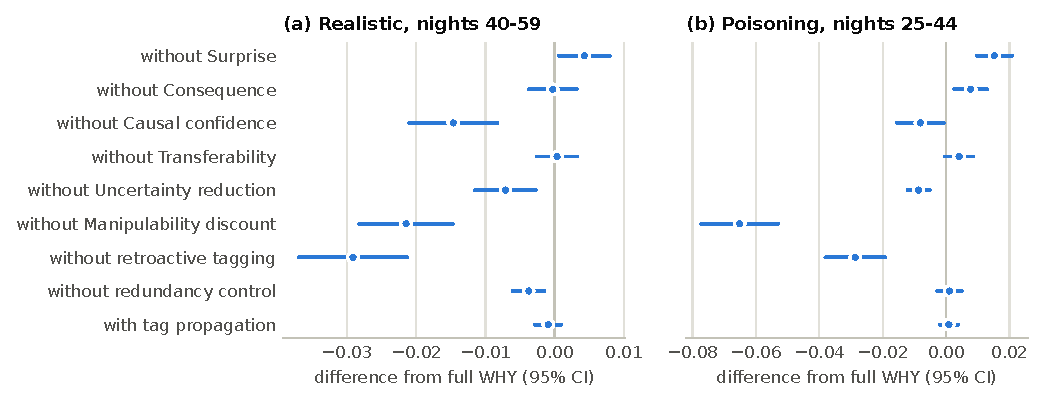
\includegraphics[width=\linewidth]{../figs/fig_ablation.pdf}
\caption{Ablations: paired difference from the full method with 95\% CIs (20 seeds). Left of zero means the component helps.}
\label{fig:ablation}
\end{figure}

\subsection{Which parts of the score matter}
\label{sec:ablations}
The ablations (Table~\ref{tab:ablation}, Figure~\ref{fig:ablation}) do not support every factor in Equation~\ref{eq:why}. The components that carried decision quality in the Realistic scenario were retroactive tagging (\val{abl-realistic-noretro-ndq_tr}), the manipulability discount (\val{abl-realistic-noM-ndq_tr}), causal confidence (\val{abl-realistic-noK-ndq_tr}), uncertainty reduction (\val{abl-realistic-noU-ndq_tr}), and redundancy control (\val{abl-realistic-nogreedy-ndq_tr}). Removing consequence (\val{abl-realistic-noC-ndq_tr}) or transferability (\val{abl-realistic-noT-ndq_tr}) made no measurable difference, and removing surprise slightly \emph{improved} decision quality (\val{abl-realistic-noS-ndq_tr}) and poison resistance (\val{abl-poison-noS-ndq_pwin} over nights 25--44).

Surprise is also where the calibration cost comes from. WHY's calibration error was \val{realistic-why-ece}, about \val{ece-ratio-why-random} times random retention's \val{realistic-random-ece}; without the surprise factor it fell to \val{noS-realistic-ece-val}, better than every capacity-limited baseline. Selecting outcomes because the model got them wrong gives the model a sample in which it is usually wrong, which shifts its probabilities even while its choices improve. Consequence raised poison intake for a related reason: honest high-stakes outcomes tend to arrive late, so same-day outcomes, including poison, look relatively consequential on the night they resolve (without the consequence factor, poison fell to \val{abl-poison-noC-poison34-val}\% of memory).

The honest summary is that what worked was \emph{when} and \emph{how far to trust} an outcome, not how dramatic it was: wait for the consequence, discount channels that can be written by interested parties, ignore days on which everything failed at once, and prefer evidence the model can still learn from. We keep Equation~\ref{eq:why} as the tested specification, because changing it now would mean tuning on evaluation seeds. A reduced score without surprise, consequence, or transferability is preregistered as a secondary arm of Experiment~2.

\begin{figure}[t]
\centering
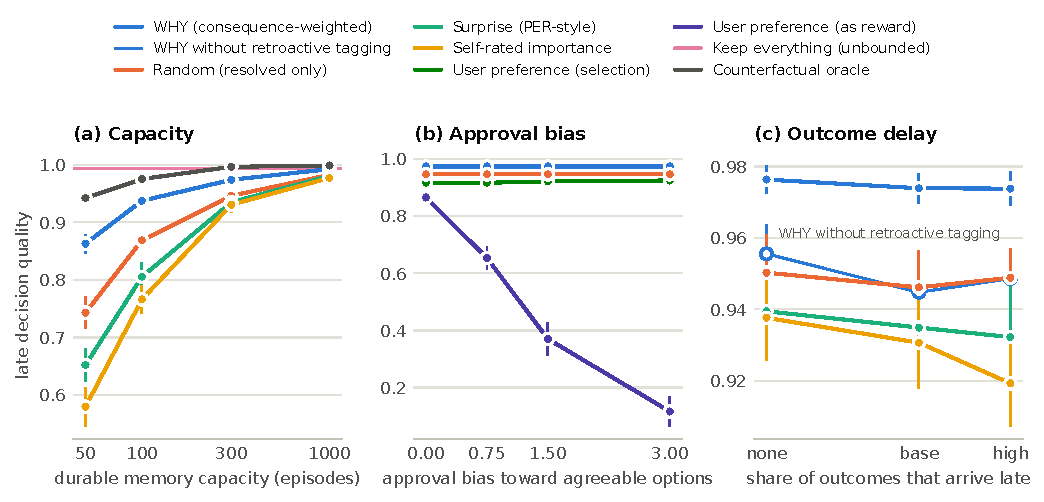
\includegraphics[width=\linewidth]{../figs/fig_sweeps.pdf}
\caption{Sweeps in the Realistic scenario (20 seeds, 95\% CIs). (a) Durable memory capacity; the horizontal line is unbounded memory. (b) Strength of the approval bias toward agreeable options. (c) Share of outcomes that resolve late (none, base rate, high). WHY and resolved-only random retention never read approval, so their lines in (b) are flat by construction.}
\label{fig:sweeps}
\end{figure}

\subsection{Capacity, approval, and delay}
\label{sec:sweeps}
\paragraph{Capacity.} The advantage of consequence-weighting grows as memory shrinks (Figure~\ref{fig:sweeps}a). At 50 engrams WHY reached \val{capsw-why-50}, against \val{capsw-random_resolved-50} for resolved-only random retention, \val{capsw-surprise-50} for PER-style surprise, and \val{capsw-importance-50} for self-rated importance. At 1{,}000 engrams, a sixth of all episodes, it reached \val{capsw-why-1000}, statistically indistinguishable from unbounded memory (\val{capsw-keep_all}; paired difference \val{pair-cap1000-keep_all}\,$\pm$\,\val{pair-cap1000-keep_all-ci}), while resolved-only random retention reached \val{capsw-random_resolved-1000}. The oracle's \val{capsw-oracle-50} at 50 engrams shows how much more a better selection rule could still recover when memory is scarce.

\paragraph{Approval bias.} Selecting episodes by approval cost roughly the same at every level of bias (\val{appr-user_pref-0.0} with no bias, \val{appr-user_pref-3.0} with strong bias), because that policy still trained on outcomes (Figure~\ref{fig:sweeps}b). Using approval as the reward collapsed as the bias grew, from \val{appr-user_pref_reward-0.0} to \val{appr-user_pref_reward-0.75}, \val{appr-user_pref_reward-1.5}, and \val{appr-user_pref_reward-3.0}. The damage comes from what a memory is trained on, more than from which memories are selected.

\paragraph{Delay.} WHY's decision quality barely moved as the share of late outcomes changed (\val{delay-why-0.0}, \val{delay-why-1.0}, \val{delay-why-1.6}; Figure~\ref{fig:sweeps}c), and neither did the value of retroactive tagging (\val{delay-retro_gap-0.0}, \val{delay-retro_gap-1.0}, \val{delay-retro_gap-1.6}). In this environment its value comes less from late outcomes specifically than from refusing to commit before any outcome exists, including the fifth of outcomes that never arrive, and from rescoring as the model changes. Self-rated importance, which commits at write time, declined as delays grew (\val{delay-importance-0.0} to \val{delay-importance-1.6}).


\subsection{Calibration and regret}
Beyond the surprise factor, selecting for decision value costs calibration in general: the oracle, which also selects for decision value, was similarly miscalibrated (\val{realistic-oracle-ece}). Online regret for WHY was \val{realistic-why-regret}\% of a random policy's, close to the oracle's \val{realistic-oracle-regret}\% and below every other capacity-limited policy, but well above unbounded memory's \val{realistic-keep_all-regret}\%, whose tighter posterior needs less exploration.

\subsection{Verdict}
Table~\ref{tab:verdict} restates the hypothesis and its parts against the evidence.
\begin{table}[H]
\centering\small
\caption{The hypothesis against the evidence from Experiment~1.}
\label{tab:verdict}
\begin{tabular}{@{}p{4.7cm}p{7.0cm}p{2.9cm}@{}}
\toprule
Claim & Evidence & Verdict\\
\midrule
Beats FIFO, similarity, recurrence, self-rated salience, and user preference under a capacity limit & positive on every seed in Realistic, Poisoning, and World change; smaller but positive in Clean & supported\\
The advantage comes from late, noisy, or manipulated outcomes & Clean gap \val{pair-clean-random-ndq_tr} vs random, Realistic \val{pair-realistic-random-ndq_tr}; noisy and manipulated channels matter, the share of late outcomes barely does & partly supported\\
The advantage grows as capacity shrinks & gap to resolved-only random: \val{capsw-why-50} vs \val{capsw-random_resolved-50} at 50 engrams; matches unbounded memory at 1{,}000 & supported\\
Robust to misleading experiences & self-report poisoning and shocks: yes; verified poisoning: admits poison at \val{pratio-poison_verified-why}$\times$ the honest rate & conditional\\
Retroactive tagging matters & largest ablation in Realistic; similar gap with or without late outcomes, so its value comes from deferral and rescoring & supported, not delay-specific\\
Every factor of the WHY score earns its place & surprise, consequence, and transferability do not in this environment & not supported\\
Bounded, selective memory beats remembering everything & only when the world changes; unbounded memory wins in every stationary scenario & not supported in stationary worlds\\
Improves calibration & worse than random retention (driven by the surprise factor) & not supported\\
\bottomrule
\end{tabular}
\end{table}
